\documentclass[twocolumn,10pt]{article}
\title{Area of Triangles}
\setlength{\columnsep}{20pt} 
\usepackage{amsmath,hyperref,cancel,graphicx}
 \def\shrinkfactor{0.55}
 \usepackage[margin=1.5cm]{geometry}
\usepackage[usenames,dvipsnames]{color}
 
 \newcommand{\blue}[1]{{\color{Blue}#1}} 
 \newcommand{\purple}[1]{{\color{Purple}#1}} 
 \newcommand{\red}[1]{{\color{Red}#1}} 
 \newcommand{\green}[1]{{\color{Green}#1}} 
 \newcommand{\gray}[1]{{\color{Gray}#1}} 
  \newcommand{\pink}[1]{{\color{Magenta}#1}}   


\begin{document}
\maketitle



\section{\href{https://www.khanacademy.org/devadmin/content/items/x1793ca122616912c}{x1793ca122616912c}}

\noindent
**Which triangle has the larger area?**  

Triangle $1$:  $\qquad\qquad \qquad ~~~~$ Triangle $2$:  

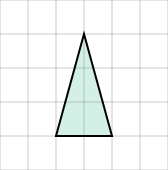
\includegraphics[scale=\shrinkfactor]{figures/de446b509a40b3e231b7217d8602d7e3d1ef4c90.png} $\quad$ 
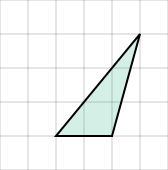
\includegraphics[scale=\shrinkfactor]{figures/dc0e8470e25253d17fd6faaff4da3897941fe7e9.png}

\paragraph{Ans} 

Triangle $1$

Triangle $2$

\fbox{ They have the same area.

}

 Not enough information



\paragraph{Hint 1}We can enclose each of the triangles in a rectangle to help us calculate the areas.  

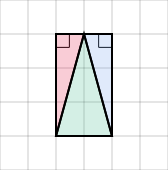
\includegraphics[scale=\shrinkfactor]{figures/fc0f214e94d78b39b2a58a88fe123e8f93a727d3.png} 
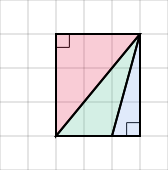
\includegraphics[scale=\shrinkfactor]{figures/dec5586c9571e1ad5901d4114bd844888463acb4.png}

\paragraph{Hint 2}The area of an original triangle can be found by subtracting the areas of the additional right triangles from the area of the enclosing rectangle.  

\paragraph{Hint 3}For Triangle $1$, the enclosing rectangle has an area of $2 \times 3 = 6$, and the areas of the two additional right triangles are:  

$\qquad \blue{\dfrac{1 \cdot 3}{2}} = \blue{1.5}$  

$\qquad \red{\dfrac{1 \cdot 3}{2}} = \red{1.5}$  

Now we can subtract the areas of the additional triangles from the area of the rectangle.

$\qquad 6-\blue1\blue.\blue5-\red{1.5}=\green{3}$  

Triangle $1$ has an area of $\green{3} \text{ units}^2$. What about Triangle $2$?

\paragraph{Hint 4}For Triangle $2$, the enclosing rectangle has an area of $3\times 3 = 9$, and the areas of the two additional right triangles are:  

$\qquad \blue{\dfrac{1 \cdot 3}{2}} = \blue{1.5}$  

$\qquad \red{\dfrac{3 \cdot 3}{2}} = \red{4.5}$  

Now we can subtract the areas of the additional triangles from the area of the rectangle.

$\qquad 9-\blue1\blue.\blue5-\red{4.5}=\green{3}$  

Triangle $2$ has an area of $\green{3} \text{ units}^2$.

\paragraph{Hint 5}Triangle $1$ and Triangle $2$ have the same area.



\medskip
\noindent
\textbf{Tags:} {\footnotesize CC.6.G.A.1, Area of Triangle 1.1, SB.6.1.H.1.SR}\\
\textbf{Version:} e107ed58.. 2013-10-15
\smallskip\hrule





\section{\href{https://www.khanacademy.org/devadmin/content/items/x3370ec68c3438ee8}{x3370ec68c3438ee8}}

\noindent
**Which triangle has the larger area?**  

Triangle $1$:  $\qquad\qquad \qquad ~~~~$ Triangle $2$:  

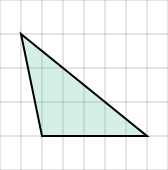
\includegraphics[scale=\shrinkfactor]{figures/dd6e582868d2bc3d35ca3f329428a4681201dfe1.png} 
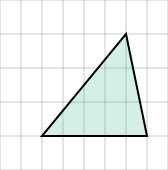
\includegraphics[scale=\shrinkfactor]{figures/a0b7bee11f79cc45ba1a5a0414484104a83a92ec.png}

\paragraph{Ans} 

Triangle $1$

Triangle $2$

\fbox{ They have the same area.

}

 Not enough information



\paragraph{Hint 1}We can enclose each of the triangles in a rectangle to help us calculate the areas.  

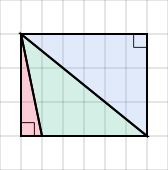
\includegraphics[scale=\shrinkfactor]{figures/654fe9a0a38e5306d6be147e41867389bd058f2d.png} 
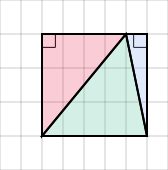
\includegraphics[scale=\shrinkfactor]{figures/48e9376d7eecdea2a460607bf78e290aedee5505.png}

\paragraph{Hint 2}The area of an original triangle can be found by subtracting the areas of the additional right triangles from the area of the enclosing rectangle.  

\paragraph{Hint 3}For Triangle $1$, the enclosing rectangle has an area of $3 \times 6 = 18$, and the areas of the two additional right triangles are:  

$\qquad \blue{\dfrac{3 \cdot 6}{2}} = \blue{9}$  

$\qquad \red{\dfrac{1 \cdot 3}{2}} = \red{1.5}$  

Now we can subtract the areas of the additional triangles from the area of the rectangle.

$\qquad 18-\blue9-\red{1.5}=\green{7.5}$  

Triangle $1$ has an area of $\green{7.5} \text{ units}^2$. What about Triangle $2$?

\paragraph{Hint 4}For Triangle $2$, the enclosing rectangle has an area of $3\times 5 = 15$, and the areas of the two additional right triangles are:  

$\qquad \blue{\dfrac{1 \cdot 3}{2}} = \blue{1.5}$  

$\qquad \red{\dfrac{3 \cdot 4}{2}} = \red{6}$  

Now we can subtract the areas of the additional triangles from the area of the rectangle.

$\qquad 15-\blue1\blue.\blue5-\red{6}=\green{7.5}$  

Triangle $2$ has an area of $\green{7.5} \text{ units}^2$.

\paragraph{Hint 5}Triangle $1$ and Triangle $2$ have the same area.



\medskip
\noindent
\textbf{Tags:} {\footnotesize CC.6.G.A.1, Area of Triangle 1.1, SB.6.1.H.1.SR}\\
\textbf{Version:} d020f305.. 2013-10-15
\smallskip\hrule





\section{\href{https://www.khanacademy.org/devadmin/content/items/x3460395511aba88f}{x3460395511aba88f}}

\noindent
**Which triangle has the larger area?**  

Triangle $1$:  $\qquad\qquad \qquad ~~~~$ Triangle $2$:  

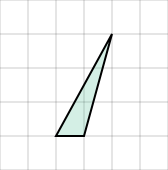
\includegraphics[scale=\shrinkfactor]{figures/c64b4d770bfcac7be00c3880806f0e6b75094446.png} $\quad$ 
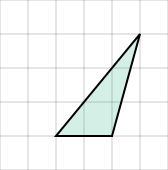
\includegraphics[scale=\shrinkfactor]{figures/dc0e8470e25253d17fd6faaff4da3897941fe7e9.png}

\paragraph{Ans} 

Triangle $1$

\fbox{ Triangle $2$

}

 They have the same area.

Not enough information



\paragraph{Hint 1}We can enclose each of the triangles in a rectangle to help us calculate the areas.  

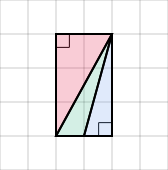
\includegraphics[scale=\shrinkfactor]{figures/4c4a94b2aca01211cb04207e5a823cc5d58570e3.png} 
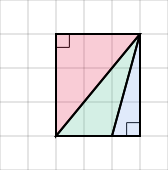
\includegraphics[scale=\shrinkfactor]{figures/dec5586c9571e1ad5901d4114bd844888463acb4.png}

\paragraph{Hint 2}The area of an original triangle can be found by subtracting the areas of the additional right triangles from the area of the enclosing rectangle.  

\paragraph{Hint 3}For Triangle $1$, the enclosing rectangle has an area of $2 \times 3 = 6$, and the areas of the two additional right triangles are:  

$\qquad \blue{\dfrac{1 \cdot 3}{2}} = \blue{1.5}$  

$\qquad \red{\dfrac{2 \cdot 3}{2}} = \red{3}$  

Now we can subtract the areas of the additional triangles from the area of the rectangle.

$\qquad 6-\blue1\blue.\blue5-\red{3}=\green{1.5}$  

Triangle $1$ has an area of $\green{1.5} \text{ units}^2$. What about Triangle $2$?

\paragraph{Hint 4}For Triangle $2$, the enclosing rectangle has an area of $3\times 3 = 9$, and the areas of the two additional right triangles are:  

$\qquad \blue{\dfrac{1 \cdot 3}{2}} = \blue{1.5}$  

$\qquad \red{\dfrac{3 \cdot 3}{2}} = \red{4.5}$  

Now we can subtract the areas of the additional triangles from the area of the rectangle.

$\qquad 9-\blue1\blue.\blue5-\red{4.5}=\green{3}$  

Triangle $2$ has an area of $\green{3} \text{ units}^2$.

\paragraph{Hint 5}Triangle $2$ has the larger area.



\medskip
\noindent
\textbf{Tags:} {\footnotesize CC.6.G.A.1, Area of Triangle 1.1, SB.6.1.H.1.SR}\\
\textbf{Version:} a90205ed.. 2013-10-15
\smallskip\hrule





\section{\href{https://www.khanacademy.org/devadmin/content/items/x4964c4a44ebbeaa5}{x4964c4a44ebbeaa5}}

\noindent
**Which triangle has the larger area?**  

Triangle $1$:  $\qquad\qquad \qquad ~~~~$ Triangle $2$:  

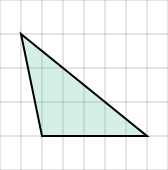
\includegraphics[scale=\shrinkfactor]{figures/dd6e582868d2bc3d35ca3f329428a4681201dfe1.png} 
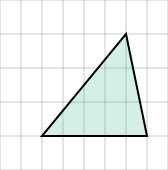
\includegraphics[scale=\shrinkfactor]{figures/a0b7bee11f79cc45ba1a5a0414484104a83a92ec.png}

\paragraph{Ans} 

Triangle $1$

Triangle $2$

\fbox{ They have the same area.

}

 Not enough information



\paragraph{Hint 1}We can enclose each of the triangles in a rectangle to help us calculate the areas.  

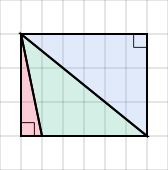
\includegraphics[scale=\shrinkfactor]{figures/654fe9a0a38e5306d6be147e41867389bd058f2d.png} 
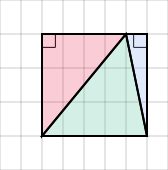
\includegraphics[scale=\shrinkfactor]{figures/48e9376d7eecdea2a460607bf78e290aedee5505.png}

\paragraph{Hint 2}The area of an original triangle can be found by subtracting the areas of the additional right triangles from the area of the enclosing rectangle.  

\paragraph{Hint 3}For Triangle $1$, the enclosing rectangle has an area of $3 \times 6 = 18$, and the areas of the two additional right triangles are:  

$\qquad \blue{\dfrac{3 \cdot 6}{2}} = \blue{9}$  

$\qquad \red{\dfrac{1 \cdot 3}{2}} = \red{1.5}$  

Now we can subtract the areas of the additional triangles from the area of the rectangle.

$\qquad 18-\blue9-\red{1.5}=\green{7.5}$  

Triangle $1$ has an area of $\green{7.5} \text{ units}^2$. What about Triangle $2$?

\paragraph{Hint 4}For Triangle $2$, the enclosing rectangle has an area of $3\times 5 = 15$, and the areas of the two additional right triangles are:  

$\qquad \blue{\dfrac{1 \cdot 3}{2}} = \blue{1.5}$  

$\qquad \red{\dfrac{3 \cdot 4}{2}} = \red{6}$  

Now we can subtract the areas of the additional triangles from the area of the rectangle.

$\qquad 15-\blue1\blue.\blue5-\red{6}=\green{7.5}$  

Triangle $2$ has an area of $\green{7.5} \text{ units}^2$.

\paragraph{Hint 5}Triangle $1$ and Triangle $2$ have the same area.



\medskip
\noindent
\textbf{Tags:} {\footnotesize CC.6.G.A.1, Area of Triangle 1.1, SB.6.1.H.1.SR}\\
\textbf{Version:} a77372c8.. 2013-10-15
\smallskip\hrule





\section{\href{https://www.khanacademy.org/devadmin/content/items/x545fee0c9a9ced8e}{x545fee0c9a9ced8e}}

\noindent
**Which triangle has the larger area?**  

Triangle $1$:  $\qquad\qquad \qquad ~~~~$ Triangle $2$:  

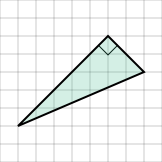
\includegraphics[scale=\shrinkfactor]{figures/46841150979f49ca89a48dfd0ca0e6f1e8e7832d.png} $\quad$ 
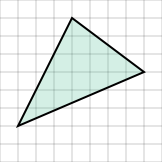
\includegraphics[scale=\shrinkfactor]{figures/3a950e606588e77f9e12097ab1e33680edb52682.png}

\paragraph{Ans} 

Triangle $1$

\fbox{ Triangle $2$

}

 They have the same area.

Not enough information



\paragraph{Hint 1}We can enclose each of the triangles in a rectangle to help us calculate the areas.  

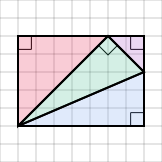
\includegraphics[scale=\shrinkfactor]{figures/007ce6e3f8950260d7c441f0203fe8adf5d08f91.png} 
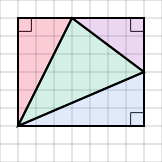
\includegraphics[scale=\shrinkfactor]{figures/e493003dc024741cbf270d5909c891c9e151ebaf.png}

\paragraph{Hint 2}The area of an original triangle can be found by subtracting the areas of the additional right triangles from the area of the enclosing rectangle.  

\paragraph{Hint 3}For Triangle $1$, the enclosing rectangle has an area of $5 \times 7 = 35$, and the areas of the three additional right triangles are:  

$\qquad \purple{\dfrac{2 \cdot 2}{2}} = \purple2$  

$\qquad \blue{\dfrac{3 \cdot 7}{2}} = \blue{10.5}$  

$\qquad \red{\dfrac{5 \cdot 5}{2}} = \red{12.5}$  

Now we can subtract the areas of the additional triangles from the area of the rectangle.

$\qquad 35-\purple2-\blue1\blue0\blue.\blue5-\red1\red2\red.\red5=\green1\green0$  

Triangle $1$ has an area of $\green{10} \text{ units}^2$. What about Triangle $2$?

\paragraph{Hint 4}For Triangle $2$, the enclosing rectangle has an area of $6 \times 7 = 42$, and the areas of the three right triangles are: 

$\qquad \purple{\dfrac{3 \cdot 4}{2}} = \purple6$  

$\qquad \blue{\dfrac{3 \cdot 7}{2}} = \blue{10.5}$  

$\qquad \red{\dfrac{3 \cdot 6}{2}} = \red{9}$  

Now we can subtract the areas of the additional triangles from the area of the rectangle.

$\qquad 42-\purple6-\blue1\blue0\blue.\blue5-\red9=\green{16.5}$  

Triangle $2$ has an area of $\green{16.5} \text{ units}^2$.

\paragraph{Hint 5}Triangle $2$ has a larger area.



\medskip
\noindent
\textbf{Tags:} {\footnotesize CC.6.G.A.1, Area of Triangle 1.1, SB.6.1.H.1.SR}\\
\textbf{Version:} 96b97490.. 2013-10-15
\smallskip\hrule





\section{\href{https://www.khanacademy.org/devadmin/content/items/x7da40cef9abd818a}{x7da40cef9abd818a}}

\noindent
**Which triangle has the larger area?**  

Triangle $1$:  $\qquad\qquad \qquad ~~~~$ Triangle $2$:  

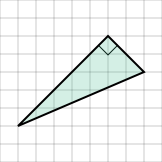
\includegraphics[scale=\shrinkfactor]{figures/46841150979f49ca89a48dfd0ca0e6f1e8e7832d.png} $\quad$ 
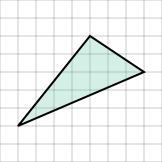
\includegraphics[scale=\shrinkfactor]{figures/8b6a988158cd3db95c5b26bd13390a3c70a2c055.png}


\paragraph{Ans} 

Triangle $1$

\fbox{ Triangle $2$

}

 They have the same area.

Not enough information



\paragraph{Hint 1}We can enclose each of the triangles in a rectangle to help us calculate the areas.  

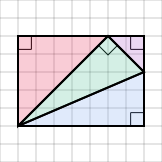
\includegraphics[scale=\shrinkfactor]{figures/007ce6e3f8950260d7c441f0203fe8adf5d08f91.png} 
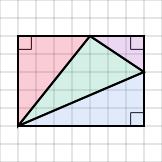
\includegraphics[scale=\shrinkfactor]{figures/8bbfecfe4fe8d5414e8abf67cdb22cdeec58672e.png}

\paragraph{Hint 2}The area of an original triangle can be found by subtracting the areas of the additional right triangles from the area of the enclosing rectangle.  

\paragraph{Hint 3}FFor Triangle $1$, the enclosing rectangle has an area of $5 \times 7 = 35$, and the areas of the three additional right triangles are:  

$\qquad \purple{\dfrac{2 \cdot 2}{2}} = \purple2$  

$\qquad \blue{\dfrac{3 \cdot 7}{2}} = \blue{10.5}$  

$\qquad \red{\dfrac{5 \cdot 5}{2}} = \red{12.5}$  

Now we can subtract the areas of the additional triangles from the area of the rectangle.

$\qquad 35-\purple2-\blue1\blue0\blue.\blue5-\red1\red2\red.\red5=\green1\green0$  

Triangle $1$ has an area of $\green{10} \text{ units}^2$. What about Triangle $2$?

\paragraph{Hint 4}For Triangle $2$, the enclosing rectangle has an area of $5 \times 7 = 35$, and the areas of the three right triangles are: 

$\qquad \purple{\dfrac{2 \cdot 3}{2}} = \purple3$  

$\qquad \blue{\dfrac{3 \cdot 7}{2}} = \blue{10.5}$  

$\qquad \red{\dfrac{4 \cdot 5}{2}} = \red{10}$  

Now we can subtract the areas of the additional triangles from the area of the rectangle.

$\qquad 35-\purple3-\blue1\blue0\blue.\blue5-\red{10}=\green{11.5}$  

Triangle $2$ has an area of $\green{11.5} \text{ units}^2$.

\paragraph{Hint 5}Triangle $2$ has a larger area.



\medskip
\noindent
\textbf{Tags:} {\footnotesize CC.6.G.A.1, Area of Triangle 1.1, SB.6.1.H.1.SR}\\
\textbf{Version:} fb9363ff.. 2013-10-15
\smallskip\hrule





\section{\href{https://www.khanacademy.org/devadmin/content/items/xb0caf8e9a6dec91f}{xb0caf8e9a6dec91f}}

\noindent
**Which triangle has the larger area?**  

Triangle $1$:  $\qquad\qquad \qquad ~~~~$ Triangle $2$:  

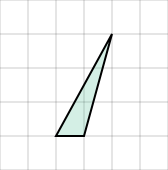
\includegraphics[scale=\shrinkfactor]{figures/c64b4d770bfcac7be00c3880806f0e6b75094446.png} $\quad$ 
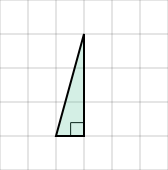
\includegraphics[scale=\shrinkfactor]{figures/a43213f31b2af310e56805358770e9ac01dfc3ce.png}

\paragraph{Ans} 

Triangle $1$

Triangle $2$

\fbox{ They have the same area.

}

 Not enough information



\paragraph{Hint 1}We can enclose each of the triangles in a rectangle to help us calculate the areas.  

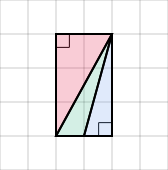
\includegraphics[scale=\shrinkfactor]{figures/4c4a94b2aca01211cb04207e5a823cc5d58570e3.png} 
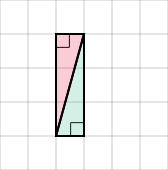
\includegraphics[scale=\shrinkfactor]{figures/9bb61a3c94f78b9667feeba29e0391bb34db147a.png}

\paragraph{Hint 2}The area of an original triangle can be found by subtracting the areas of the additional right triangles from the area of the enclosing rectangle.  

\paragraph{Hint 3}For Triangle $1$, the enclosing rectangle has an area of $2 \times 3 = 6$, and the areas of the two additional right triangles are:  

$\qquad \blue{\dfrac{1 \cdot 3}{2}} = \blue{1.5}$  

$\qquad \red{\dfrac{2 \cdot 3}{2}} = \red{3}$  

Now we can subtract the areas of the additional triangles from the area of the rectangle.

$\qquad 6-\blue1\blue.\blue5-\red3=\green{1.5}$  

Triangle $1$ has an area of $\green{1.5} \text{ units}^2$. What about Triangle $2$?

\paragraph{Hint 4}For Triangle $2$, the enclosing rectangle has an area of $3\times 1 = 3$, and the area of the right triangle is:  

$\qquad \red{\dfrac{1 \cdot 3}{2}} = \red{1.5}$  

Now we can subtract the areas of the additional triangle from the area of the rectangle.

$\qquad 3-\red{1.5}=\green{1.5}$  

Triangle $2$ has an area of $\green{1.5} \text{ units}^2$.

\paragraph{Hint 5}Triangle $1$ and Triangle $2$ have the same area.



\medskip
\noindent
\textbf{Tags:} {\footnotesize CC.6.G.A.1, Area of Triangle 1.1, SB.6.1.H.1.SR}\\
\textbf{Version:} eb4fe914.. 2013-10-15
\smallskip\hrule





\section{\href{https://www.khanacademy.org/devadmin/content/items/xb6b2062e3175da4d}{xb6b2062e3175da4d}}

\noindent
**Which triangle has the larger area?**  

Triangle $1$:  $\qquad\qquad \qquad ~~~~$ Triangle $2$:  

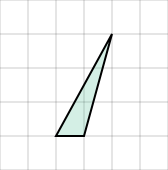
\includegraphics[scale=\shrinkfactor]{figures/c64b4d770bfcac7be00c3880806f0e6b75094446.png} $\quad$ 
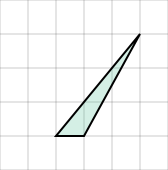
\includegraphics[scale=\shrinkfactor]{figures/7bc1f0ff36ec2f690538dfcf8a0d75bdc3484d55.png}

\paragraph{Ans} 

Triangle $1$

Triangle $2$

\fbox{ They have the same area.

}

 Not enough information



\paragraph{Hint 1}We can enclose each of the triangles in a rectangle to help us calculate the areas.  

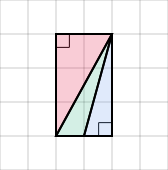
\includegraphics[scale=\shrinkfactor]{figures/4c4a94b2aca01211cb04207e5a823cc5d58570e3.png} 
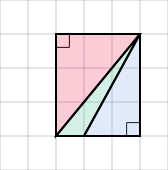
\includegraphics[scale=\shrinkfactor]{figures/7d48421a544149b3e928997e62b20245c13ac51e.png}

\paragraph{Hint 2}The area of an original triangle can be found by subtracting the areas of the additional right triangles from the area of the enclosing rectangle.  

\paragraph{Hint 3}For Triangle $1$, the enclosing rectangle has an area of $2 \times 3 = 6$, and the areas of the two additional right triangles are:  

$\qquad \blue{\dfrac{1 \cdot 3}{2}} = \blue{1.5}$  

$\qquad \red{\dfrac{2 \cdot 3}{2}} = \red{3}$  

Now we can subtract the areas of the additional triangles from the area of the rectangle.

$\qquad 6-\blue1\blue.\blue5-\red3=\green{1.5}$  

Triangle $1$ has an area of $\green{1.5} \text{ units}^2$. What about Triangle $2$?

\paragraph{Hint 4}For Triangle $2$, the enclosing rectangle has an area of $3\times 3 = 9$, and the areas of the two additional right triangles are:  

$\qquad \blue{\dfrac{2 \cdot 3}{2}} = \blue{3}$  

$\qquad \red{\dfrac{3 \cdot 3}{2}} = \red{4.5}$  

Now we can subtract the areas of the additional triangles from the area of the rectangle.

$\qquad 9-\blue3-\red{4.5}=\green{1.5}$  

Triangle $2$ has an area of $\green{1.5} \text{ units}^2$.

\paragraph{Hint 5}Triangle $1$ and Triangle $2$ have the same area.



\medskip
\noindent
\textbf{Tags:} {\footnotesize CC.6.G.A.1, Area of Triangle 1.1, SB.6.1.H.1.SR}\\
\textbf{Version:} 58d35ba4.. 2013-10-15
\smallskip\hrule





\section{\href{https://www.khanacademy.org/devadmin/content/items/xc81137bfb1ce5ecb}{xc81137bfb1ce5ecb}}

\noindent
**Which triangle has the larger area?**  

Triangle $1$:  $\qquad\qquad \qquad ~~~~$ Triangle $2$:  

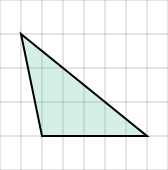
\includegraphics[scale=\shrinkfactor]{figures/dd6e582868d2bc3d35ca3f329428a4681201dfe1.png} 
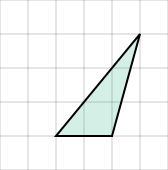
\includegraphics[scale=\shrinkfactor]{figures/dc0e8470e25253d17fd6faaff4da3897941fe7e9.png}

\paragraph{Ans} 

\fbox{ Triangle $1$

}

 Triangle $2$

They have the same area.

Not enough information



\paragraph{Hint 1}We can enclose each of the triangles in a rectangle to help us calculate the areas.  

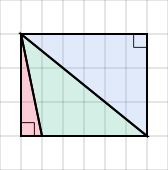
\includegraphics[scale=\shrinkfactor]{figures/654fe9a0a38e5306d6be147e41867389bd058f2d.png} 
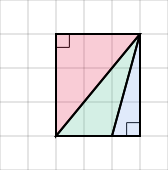
\includegraphics[scale=\shrinkfactor]{figures/dec5586c9571e1ad5901d4114bd844888463acb4.png}

\paragraph{Hint 2}The area of an original triangle can be found by subtracting the areas of the additional right triangles from the area of the enclosing rectangle.  

\paragraph{Hint 3}For Triangle $1$, the enclosing rectangle has an area of $3 \times 6 = 18$, and the areas of the two additional right triangles are:  

$\qquad \blue{\dfrac{3 \cdot 6}{2}} = \blue{9}$  

$\qquad \red{\dfrac{1 \cdot 3}{2}} = \red{1.5}$  

Now we can subtract the areas of the additional triangles from the area of the rectangle.

$\qquad 18-\blue9-\red{1.5}=\green{7.5}$  

Triangle $1$ has an area of $\green{7.5} \text{ units}^2$. What about Triangle $2$?

\paragraph{Hint 4}For Triangle $2$, the enclosing rectangle has an area of $3\times 3 = 9$, and the areas of the two additional right triangles are:  

$\qquad \blue{\dfrac{1 \cdot 3}{2}} = \blue{1.5}$  

$\qquad \red{\dfrac{3 \cdot 3}{2}} = \red{4.5}$  

Now we can subtract the areas of the additional triangles from the area of the rectangle.

$\qquad 9-\blue1\blue.\blue5-\red{4.5}=\green{3}$  

Triangle $2$ has an area of $\green{3} \text{ units}^2$.

\paragraph{Hint 5}Triangle $1$ has the larger area.



\medskip
\noindent
\textbf{Tags:} {\footnotesize CC.6.G.A.1, Area of Triangle 1.1, SB.6.1.H.1.SR}\\
\textbf{Version:} c2178db8.. 2013-10-15
\smallskip\hrule





\section{\href{https://www.khanacademy.org/devadmin/content/items/xe6b2fe97c9c92959}{xe6b2fe97c9c92959}}

\noindent
**Which triangle has the larger area?**  

Triangle $1$:  $\qquad\qquad \qquad ~~~~$ Triangle $2$:  

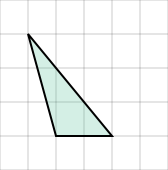
\includegraphics[scale=\shrinkfactor]{figures/9f2002eedd62178a3ce9e26198e205d26342422f.png}$\quad$ 
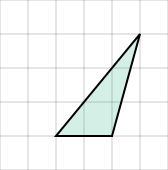
\includegraphics[scale=\shrinkfactor]{figures/dc0e8470e25253d17fd6faaff4da3897941fe7e9.png}

\paragraph{Ans} 

Triangle $1$

Triangle $2$

\fbox{ They have the same area.

}

 Not enough information



\paragraph{Hint 1}We can enclose each of the triangles in a rectangle to help us calculate the areas.  

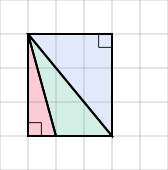
\includegraphics[scale=\shrinkfactor]{figures/0a84a76814d7f948246912f03337d59073d9bb2a.png} 
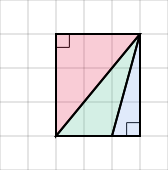
\includegraphics[scale=\shrinkfactor]{figures/dec5586c9571e1ad5901d4114bd844888463acb4.png}

\paragraph{Hint 2}The area of an original triangle can be found by subtracting the areas of the additional right triangles from the area of the enclosing rectangle.  

\paragraph{Hint 3}For Triangle $1$, the enclosing rectangle has an area of $3 \times 3 = 9$, and the areas of the two additional right triangles are:  

$\qquad \blue{\dfrac{3 \cdot 3}{2}} = \blue{4.5}$  

$\qquad \red{\dfrac{1 \cdot 3}{2}} = \red{1.5}$  

Now we can subtract the areas of the additional triangles from the area of the rectangle.

$\qquad 9-\blue4\blue.\blue5-\red{1.5}=\green{3}$  

Triangle $1$ has an area of $\green{3} \text{ units}^2$. What about Triangle $2$?

\paragraph{Hint 4}For Triangle $2$, the enclosing rectangle has an area of $3\times 3 = 9$, and the areas of the two additional right triangles are:  

$\qquad \blue{\dfrac{1 \cdot 3}{2}} = \blue{1.5}$  

$\qquad \red{\dfrac{3 \cdot 3}{2}} = \red{4.5}$  

Now we can subtract the areas of the additional triangle from the area of the rectangle.

$\qquad 9-\blue1\blue.\blue5-\red{4.5}=\green{3}$  

Triangle $2$ has an area of $\green{3} \text{ units}^2$.

\paragraph{Hint 5}Triangle $1$ and Triangle $2$ have the same area.



\medskip
\noindent
\textbf{Tags:} {\footnotesize CC.6.G.A.1, Area of Triangle 1.1, SB.6.1.H.1.SR}\\
\textbf{Version:} 7e93f912.. 2013-10-15
\smallskip\hrule





\section{\href{https://www.khanacademy.org/devadmin/content/items/xfa691da601125822}{xfa691da601125822}}

\noindent
**Which triangle has the larger area?**  

Triangle $1$:  $\qquad\qquad \qquad ~~~~$ Triangle $2$:  

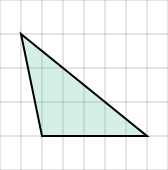
\includegraphics[scale=\shrinkfactor]{figures/dd6e582868d2bc3d35ca3f329428a4681201dfe1.png} 
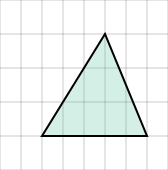
\includegraphics[scale=\shrinkfactor]{figures/4af26efe54ffe4cf7d507b8af62793c7322d6f53.png}

\paragraph{Ans} 

Triangle $1$

Triangle $2$

\fbox{ They have the same area.

}

 Not enough information



\paragraph{Hint 1}We can enclose each of the triangles in a rectangle to help us calculate the areas.  

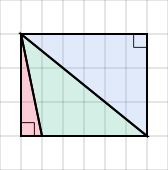
\includegraphics[scale=\shrinkfactor]{figures/654fe9a0a38e5306d6be147e41867389bd058f2d.png} 
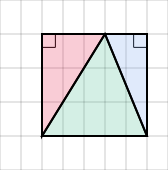
\includegraphics[scale=\shrinkfactor]{figures/7384f2bca82e3eef65f9b516b08b392a0a3da559.png}

\paragraph{Hint 2}The area of an original triangle can be found by subtracting the areas of the additional right triangles from the area of the enclosing rectangle.  

\paragraph{Hint 3}For Triangle $1$, the enclosing rectangle has an area of $3 \times 6 = 18$, and the areas of the two additional right triangles are:  

$\qquad \blue{\dfrac{3 \cdot 6}{2}} = \blue{9}$  

$\qquad \red{\dfrac{1 \cdot 3}{2}} = \red{1.5}$  

Now we can subtract the areas of the additional triangles from the area of the rectangle.

$\qquad 18-\blue9-\red{1.5}=\green{7.5}$  

Triangle $1$ has an area of $\green{7.5} \text{ units}^2$. What about Triangle $2$?

\paragraph{Hint 4}For Triangle $2$, the enclosing rectangle has an area of $3\times 5 = 15$, and the areas of the two additional right triangles are:  

$\qquad \blue{\dfrac{2 \cdot 3}{2}} = \blue{3}$  

$\qquad \red{\dfrac{3 \cdot 3}{2}} = \red{4.5}$  

Now we can subtract the areas of the additional triangles from the area of the rectangle.

$\qquad 15-\blue3-\red{4.5}=\green{7.5}$  

Triangle $2$ has an area of $\green{7.5} \text{ units}^2$.

\paragraph{Hint 5}Triangle $1$ and Triangle $2$ have the same area.



\medskip
\noindent
\textbf{Tags:} {\footnotesize CC.6.G.A.1, Area of Triangle 1.1, SB.6.1.H.1.SR}\\
\textbf{Version:} fc7c17b1.. 2013-10-15
\smallskip\hrule





\section{\href{https://www.khanacademy.org/devadmin/content/items/x10ae6a535164e8ee}{x10ae6a535164e8ee}}

\noindent
**What is the area of the triangle below?**  


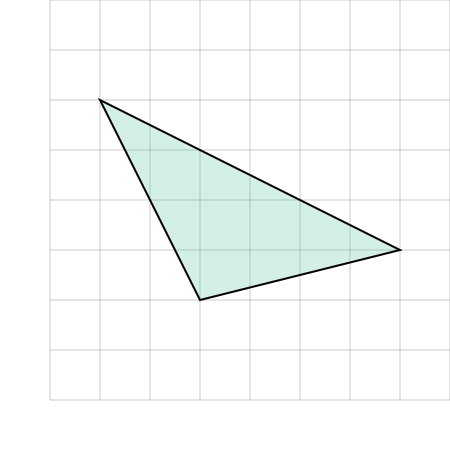
\includegraphics[scale=\shrinkfactor]{figures/f106ebaafe03d69cdae7e1cefc0501c437c31a98.png}

\paragraph{Ans} [[? input-number 1]] $\text{ units}^2$  9

\paragraph{Hint 1}We can enclose this triangle in a rectangle with area $6 \times 4 =24$.   

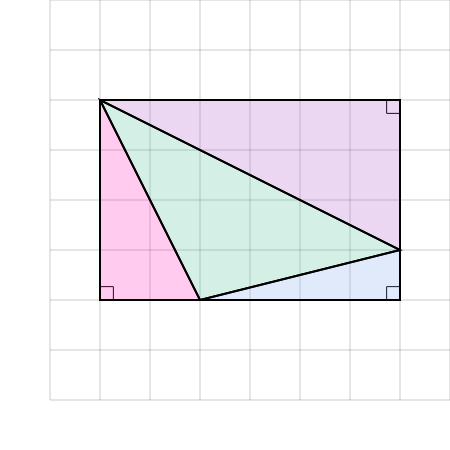
\includegraphics[scale=\shrinkfactor]{figures/f8742902f351b5e757353f5b87652f60dc589176.png}

\paragraph{Hint 2}The areas of the three additional right triangles are:  

$\qquad \purple{\dfrac{3 \cdot 6}{2}} = \purple9$  

$\qquad \blue{\dfrac{1 \cdot 4}{2}} = \blue{2}$  

$\qquad \red{\dfrac{2 \cdot 4}{2}} = \red{4}$

\paragraph{Hint 3}The area of the original triangle can be found by subtracting the area of the additional right triangles from the area of the rectangle.  

$24-\purple9-\blue2-\red4=\green{9}$

\paragraph{Hint 4}The original triangle has an area of $9 \text{ units}^2$.



\medskip
\noindent
\textbf{Tags:} {\footnotesize CC.6.G.A.1, Area of Triangle 1.2, SB.6.1.H.1.CR}\\
\textbf{Version:} acb63299.. 2013-10-15
\smallskip\hrule





\section{\href{https://www.khanacademy.org/devadmin/content/items/x39cafa2f0f4b797d}{x39cafa2f0f4b797d}}

\noindent
**What is the area of Triangle $ABC$ below?**  
All sides lengths are measured in feet.   


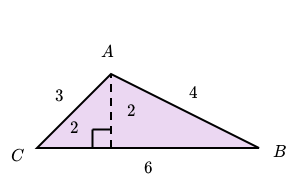
\includegraphics[scale=\shrinkfactor]{figures/d75c755c2a17646a755101119c0e83ce22d1dd70.png}

\paragraph{Ans} [[? input-number 1]] $\text { ft}^2$  6

\paragraph{Hint 1}The triangle is half of a rectangle that has a length of $6\text{ feet}$ and a width of $2\text{ feet}$.  


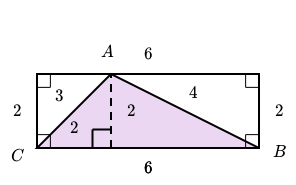
\includegraphics[scale=\shrinkfactor]{figures/665fb2b69a0eb85a287f91beb815333aa632babb.png}

\paragraph{Hint 2}It's a little easier to see that the triangle is half of the rectangle if we split the original triangle into two right triangles.

\paragraph{Hint 3}
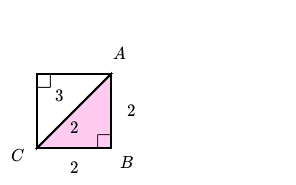
\includegraphics[scale=\shrinkfactor]{figures/86e3a05dd926e87134daef9a1aca877700f06049.png}  

This right triangle is half of a square with area $\pink2\times\pink2=\pink{4}$ $\text { ft}^2$, so this right triangle has an area of $\pink{2}\text { ft}^2$.  

\paragraph{Hint 4}
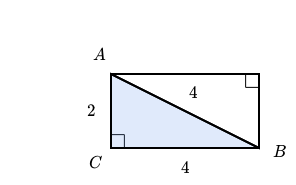
\includegraphics[scale=\shrinkfactor]{figures/1dc582bc07a6f233e01b71e6b743390c41d7b811.png}  
The other right triangle is half of a rectangle with area $\blue4\times\blue2=\blue{8}$ $\text { ft}^2$, so the other right triangle also has an area of $\blue{4}\text { ft}^2$. 

\paragraph{Hint 5}Adding the two pieces together, we see that the area is $\pink{2} + \blue{4} = \purple{6}\text { ft}^2$. 

\paragraph{Hint 6}The triangle has an area of $6\text { ft}^2$.



\medskip
\noindent
\textbf{Tags:} {\footnotesize CC.6.G.A.1, Area of Triangle 1.2, SB.6.1.H.1.CR}\\
\textbf{Version:} 5a1febb0.. 2013-10-13
\smallskip\hrule





\section{\href{https://www.khanacademy.org/devadmin/content/items/x43322953ff4acf5b}{x43322953ff4acf5b}}

\noindent
**What is the area of Triangle $ABC$ below?**  
All sides lengths are measured in feet.  


\includegraphics[scale=\shrinkfactor]{figures/b6d07b651ba10b8353bb647b4ad4d2569d28513e.png}

\paragraph{Ans} [[? input-number 1]] $\text { ft}^2$  12

\paragraph{Hint 1}The triangle is half of a rectangle that has a length of $6\text{ feet}$ and a width of $4\text{ feet}$.  


\includegraphics[scale=\shrinkfactor]{figures/b72d774061159cf67d86cdaf43d03779603fb98d.png}

\paragraph{Hint 2}It's a little easier to see that the triangle is half of the rectangle if we split the original triangle into two right triangles.

\paragraph{Hint 3}
\includegraphics[scale=\shrinkfactor]{figures/fa6ede27a1e8d5bcd4b48596b0071a26c6000849.png}  
  
This right triangle is half of a rectangle with area $\pink4\times\pink3=\pink1\pink2$ $\text { ft}^2$, so this right triangle has an area of $\pink6\text { ft}^2$.  

\paragraph{Hint 4}
\includegraphics[scale=\shrinkfactor]{figures/88674c4bd7c0ae013515f199b2ccdd0fc658a913.png}    
The other right triangle is also half of a rectangle with $\blue4\times\blue3=\blue1\blue2$ $\text { ft}^2$, so the other right triangle also has an area of $\blue6\text { ft}^2$. 

\paragraph{Hint 5}Adding the two pieces together, we see that the area is $\pink6 + \blue6 = \purple1\purple2\text { ft}^2$. 

\paragraph{Hint 6}The triangle has an area of $12\text { ft}^2$.



\medskip
\noindent
\textbf{Tags:} {\footnotesize CC.6.G.A.1, Area of Triangle 1.2, SB.6.1.H.1.CR}\\
\textbf{Version:} 069a19cf.. 2013-10-11
\smallskip\hrule





\section{\href{https://www.khanacademy.org/devadmin/content/items/x599468861ee68b78}{x599468861ee68b78}}

\noindent
**What is the area of the triangle below?**  


\includegraphics[scale=\shrinkfactor]{figures/027b98230cfeb2f7ef1f0c29da18b646763291f2.png}

\paragraph{Ans} [[? input-number 1]] $\text{ units}^2$  13

\paragraph{Hint 1}We can enclose this triangle in a rectangle with area $7 \times 4 =28$.   

\includegraphics[scale=\shrinkfactor]{figures/3c55e6c7b02fb352ff31b1b707c380e87a0b5b02.png}

\paragraph{Hint 2}The areas of the three additional right triangles are:  

$\qquad \purple{\dfrac{3 \cdot 5}{2}} = \purple{7.5}$  

$\qquad \blue{\dfrac{1 \cdot 7}{2}} = \blue{3.5}$  

$\qquad \red{\dfrac{2 \cdot 4}{2}} = \red{4}$

\paragraph{Hint 3}The area of the original triangle can be found by subtracting the area of the additional right triangles from the area of the rectangle.  

$28-\purple{7.5}-\blue{3.5}-\red4=\green{13}$

\paragraph{Hint 4}The original triangle has an area of $13 \text{ units}^2$.



\medskip
\noindent
\textbf{Tags:} {\footnotesize CC.6.G.A.1, Area of Triangle 1.2, SB.6.1.H.1.CR}\\
\textbf{Version:} c3e4c245.. 2013-10-15
\smallskip\hrule





\section{\href{https://www.khanacademy.org/devadmin/content/items/x64ba6e1bf7bb9781}{x64ba6e1bf7bb9781}}

\noindent
**What is the area of Triangle $ABC$ below?**  
All sides lengths are measured in feet.  


\includegraphics[scale=\shrinkfactor]{figures/b71b01f20084080f9539ddb8611b64c0179d65ee.png}

\paragraph{Ans} [[? input-number 1]] $\text { ft}^2$  7.5

\paragraph{Hint 1}The triangle is half of a rectangle that has a length of $5\text{ feet}$ and a width of $3\text{ feet}$.  


\includegraphics[scale=\shrinkfactor]{figures/52cec5a0b6beb585993d83b5db9d6277e893f3ab.png}

\paragraph{Hint 2}It's a little easier to see that the triangle is half of the rectangle if we split the original triangle into two right triangles.

\paragraph{Hint 3}
\includegraphics[scale=\shrinkfactor]{figures/d080cc934713ec55a885f0c66be7a4488d2568a1.png}  
  
This right triangle is half of a rectangle with area $\pink3\times\pink2=\pink{6}$ $\text { ft}^2$, so this right triangle has an area of $\pink{3}\text { ft}^2$.  

\paragraph{Hint 4}
\includegraphics[scale=\shrinkfactor]{figures/42f99e3fe6ba0529ccdf3a83750a35cf4d7e878a.png}  
The other right triangle is half of a square with area $\blue3\times\blue3=\blue{9}$ $\text { ft}^2$, so the other right triangle also has an area of $\blue{4.5}\text { ft}^2$. 

\paragraph{Hint 5}Adding the two pieces together, we see that the area is $\pink{3} + \blue{4.5} = \purple{7.5}\text { ft}^2$. 

\paragraph{Hint 6}The triangle has an area of $7.5\text { ft}^2$.



\medskip
\noindent
\textbf{Tags:} {\footnotesize CC.6.G.A.1, Area of Triangle 1.2, SB.6.1.H.1.CR}\\
\textbf{Version:} 3fa4bafa.. 2013-10-13
\smallskip\hrule





\section{\href{https://www.khanacademy.org/devadmin/content/items/x7720fa616a7c50ad}{x7720fa616a7c50ad}}

\noindent
**What is the area of the triangle below?**  


\includegraphics[scale=\shrinkfactor]{figures/992f3f54101ec07ac574037aa344e1713ad8143d.png}

\paragraph{Ans} [[? input-number 1]] $\text{ units}^2$  10

\paragraph{Hint 1}We can enclose this triangle in a rectangle with area $7 \times 5 =35$.   

\includegraphics[scale=\shrinkfactor]{figures/bd87687fd50cd1ccc88ac38f14b4f8289e2cb00b.png}  

\paragraph{Hint 2}The areas of the three additional right triangles are:  

$\qquad \purple{\dfrac{2 \cdot 2}{2}} = \purple2$  

$\qquad \blue{\dfrac{3 \cdot 7}{2}} = \blue{10.5}$  

$\qquad \red{\dfrac{5 \cdot 5}{2}} = \red{12.5}$

\paragraph{Hint 3}The area of the original triangle can be found by subtracting the area of the additional right triangles from the area of the rectangle.  

$35-\purple2-\blue1\blue0\blue.\blue5-\red1\red2\red.\red5=\green1\green0$

\paragraph{Hint 4}The original triangle has an area of $10 \text{ units}^2$.



\medskip
\noindent
\textbf{Tags:} {\footnotesize CC.6.G.A.1, Area of Triangle 1.2, SB.6.1.H.1.CR}\\
\textbf{Version:} 5d81dce5.. 2013-10-14
\smallskip\hrule





\section{\href{https://www.khanacademy.org/devadmin/content/items/x77adf2fae5d65eb7}{x77adf2fae5d65eb7}}

\noindent
**What is the area of the triangle below?**  


\includegraphics[scale=\shrinkfactor]{figures/a9d08fe8d0959ab75ff5e068e4884e2fca910183.png}

\paragraph{Ans} [[? input-number 1]] $\text{ units}^2$  7

\paragraph{Hint 1}We can enclose this triangle in a square with area $4 \times 4 =16$.   

\includegraphics[scale=\shrinkfactor]{figures/3a3c9cd9e3ded8e936dd68b236f227db7d7b7994.png}

\paragraph{Hint 2}The areas of the three additional right triangles are:  

$\qquad \purple{\dfrac{2 \cdot 3}{2}} = \purple{3}$  

$\qquad \blue{\dfrac{1 \cdot 4}{2}} = \blue{2}$  

$\qquad \red{\dfrac{2 \cdot 4}{2}} = \red{4}$

\paragraph{Hint 3}The area of the original triangle can be found by subtracting the area of the additional right triangles from the area of the square.  

$16-\purple{3}-\blue{2}-\red4=\green{7}$

\paragraph{Hint 4}The original triangle has an area of $7 \text{ units}^2$.



\medskip
\noindent
\textbf{Tags:} {\footnotesize CC.6.G.A.1, Area of Triangle 1.2, SB.6.1.H.1.CR}\\
\textbf{Version:} 200a0956.. 2013-10-15
\smallskip\hrule





\section{\href{https://www.khanacademy.org/devadmin/content/items/x98290a8f0805fe87}{x98290a8f0805fe87}}

\noindent
**What is the area of the triangle below?**  
 

\includegraphics[scale=\shrinkfactor]{figures/3899ff88992da95c7bfacc512623dc392e4a29cf.png}

\paragraph{Ans} [[? input-number 1]] $\text{ units}^2$  19.5

\paragraph{Hint 1}We can enclose this triangle in a rectangle with area $7 \times 6 =42$.   

\includegraphics[scale=\shrinkfactor]{figures/f64af607e75e5e16d10d835743b842c3e3d8ede4.png}  

\paragraph{Hint 2}The areas of the three additional right triangles are:  

$\qquad \purple{\dfrac{3 \cdot 6}{2}} = \purple9$  

$\qquad \blue{\dfrac{3 \cdot 7}{2}} = \blue{10.5}$  

$\qquad \red{\dfrac{1 \cdot 6}{2}} = \red{3}$

\paragraph{Hint 3}The area of the original triangle can be found by subtracting the area of the additional right triangles from the area of the rectangle.  

$42-\purple9-\blue1\blue0\blue.\blue5-\red3=\green{19.5}$

\paragraph{Hint 4}The  original triangle has an area of $19.5 \text{ units}^2$.



\medskip
\noindent
\textbf{Tags:} {\footnotesize CC.6.G.A.1, Area of Triangle 1.2, SB.6.1.H.1.CR}\\
\textbf{Version:} 2461bfb6.. 2013-10-15
\smallskip\hrule





\section{\href{https://www.khanacademy.org/devadmin/content/items/x9ecb73e3e695cec9}{x9ecb73e3e695cec9}}

\noindent
**What is the area of Triangle $ABC$ below?**  
All sides lengths are measured in feet.  


\includegraphics[scale=\shrinkfactor]{figures/1d918c5a96ec2027125b880b5f332b4564134beb.png}

\paragraph{Ans} [[? input-number 1]] $\text { ft}^2$  6

\paragraph{Hint 1}The triangle is half of a rectangle that has a length of $6\text{ feet}$ and a width of $2\text{ feet}$.  



\includegraphics[scale=\shrinkfactor]{figures/f92f863cca1091392224b0a6c95d7afcab9eb2bd.png}

\paragraph{Hint 2}It's a little easier to see that the triangle is half of the rectangle if we split the original triangle into two right triangles.

\paragraph{Hint 3}
\includegraphics[scale=\shrinkfactor]{figures/5e42f052bed4c0f85ed36d1bdd1c16176eb04c7a.png}  
  
This right triangle is half of a rectangle with area $\pink4\times\pink2=\pink{8}$ $\text { ft}^2$, so this right triangle has an area of $\pink{4}\text { ft}^2$.  

\paragraph{Hint 4}
\includegraphics[scale=\shrinkfactor]{figures/c892f40fcf029c387aa086d58b74f661bba173e6.png}  

The other right triangle is half of a square with area $\blue2\times\blue2=\blue{4}$ $\text { ft}^2$, so the other right triangle also has an area of $\blue{2}\text { ft}^2$. 

\paragraph{Hint 5}Adding the two pieces together, we see that the area is $\pink{4} + \blue{2} = \purple{6}\text { ft}^2$. 

\paragraph{Hint 6}The triangle has an area of $6\text { ft}^2$.



\medskip
\noindent
\textbf{Tags:} {\footnotesize CC.6.G.A.1, Area of Triangle 1.2, SB.6.1.H.1.CR}\\
\textbf{Version:} c0cfb580.. 2013-10-13
\smallskip\hrule





\section{\href{https://www.khanacademy.org/devadmin/content/items/xa171035eb92f1d61}{xa171035eb92f1d61}}

\noindent
**What is the area of the triangle below?**  


\includegraphics[scale=\shrinkfactor]{figures/817e4d036011ef1f48d458d530d4165a9e86f1cd.png}

\paragraph{Ans} [[? input-number 1]] $\text{ units}^2$  13.5

\paragraph{Hint 1}We can enclose this triangle in a rectangle with area $7 \times 4 =28$.   

\includegraphics[scale=\shrinkfactor]{figures/8bc90eb7c18be948f62cb153230a01d962de2956.png}

\paragraph{Hint 2}The areas of the three additional right triangles are:  

$\qquad \purple{\dfrac{3 \cdot 6}{2}} = \purple{9}$  

$\qquad \blue{\dfrac{1 \cdot 7}{2}} = \blue{3.5}$  

$\qquad \red{\dfrac{1 \cdot 4}{2}} = \red{2}$

\paragraph{Hint 3}The area of the original triangle can be found by subtracting the area of the additional  right triangles from the area of the rectangle.  

$28-\purple{9}-\blue{3.5}-\red2=\green{13.5}$

\paragraph{Hint 4}The original triangle has an area of $13.5 \text{ units}^2$.



\medskip
\noindent
\textbf{Tags:} {\footnotesize CC.6.G.A.1, Area of Triangle 1.2, SB.6.1.H.1.CR}\\
\textbf{Version:} 1a858c9b.. 2013-10-15
\smallskip\hrule





\section{\href{https://www.khanacademy.org/devadmin/content/items/xaac6b55019ebdd1b}{xaac6b55019ebdd1b}}

\noindent
**What is the area of Triangle $ABC$ below?**  
All sides lengths are measured in feet.  


\includegraphics[scale=\shrinkfactor]{figures/3a90146fc5362572c5ad0fa821a46373bb67ecf8.png}

\paragraph{Ans} [[? input-number 1]] $\text { ft}^2$  15

\paragraph{Hint 1}The triangle is half of a rectangle that has a length of $6\text{ feet}$ and a width of $5\text{ feet}$.  


\includegraphics[scale=\shrinkfactor]{figures/465c4efe535b5f7bd3aed911ef0d3d9f41f810a8.png}

\paragraph{Hint 2}It's a little easier to see that the triangle is half of the rectangle if we split the original triangle into two right triangles.

\paragraph{Hint 3}
\includegraphics[scale=\shrinkfactor]{figures/4bd11133bfccf53f69cadf1cc2b6a4240515eefd.png}  
  
This right triangle is half of a rectangle with area $\pink5\times\pink4=\pink{20}$ $\text { ft}^2$, so this right triangle has an area of $\pink{10}\text { ft}^2$.  

\paragraph{Hint 4}
\includegraphics[scale=\shrinkfactor]{figures/78d33707756e1a03adbea9c2a1dfd044ed47733a.png}  

The other right triangle is also half of a rectangle with area $\blue5\times\blue2=\blue{10}$ $\text { ft}^2$, so the other right triangle also has an area of $\blue{5}\text { ft}^2$. 

\paragraph{Hint 5}Adding the two pieces together, we see that the area is $\pink{10} + \blue{5} = \purple{15}\text { ft}^2$. 

\paragraph{Hint 6}The triangle has an area of $15\text { ft}^2$.



\medskip
\noindent
\textbf{Tags:} {\footnotesize CC.6.G.A.1, Area of Triangle 1.2, SB.6.1.H.1.CR}\\
\textbf{Version:} b72d8127.. 2013-10-13
\smallskip\hrule





\section{\href{https://www.khanacademy.org/devadmin/content/items/xad0626bc47031702}{xad0626bc47031702}}

\noindent
**What is the area of Triangle $ABC$ below?**  
All sides lengths are measured in feet.  


\includegraphics[scale=\shrinkfactor]{figures/8a71007892ebd84375220fdd584853f8ddbab9d3.png}

\paragraph{Ans} [[? input-number 1]] $\text { ft}^2$  12

\paragraph{Hint 1}The triangle is half of a rectangle that has a length of $6\text{ feet}$ and a width of $4\text{ feet}$.  


\includegraphics[scale=\shrinkfactor]{figures/b42be22c22a8d9a24cb327eecb3a276ac3ed9f2b.png}

\paragraph{Hint 2}It's a little easier to see that the triangle is half of the rectangle if we split the original triangle into two right triangles.

\paragraph{Hint 3}
\includegraphics[scale=\shrinkfactor]{figures/0f7ed39dbfac86b0e24274c551873f74647bb566.png}  
  
This right triangle is half of a square with area $\pink4\times\pink4=\pink{16}$ $\text { ft}^2$, so this right triangle has an area of $\pink{8}\text { ft}^2$.  

\paragraph{Hint 4}
\includegraphics[scale=\shrinkfactor]{figures/9b853964b658d5d0066616a8394d7fa928b0191d.png}  

The other right triangle is half of a rectangle with area $\blue4\times\blue2=\blue{8}$ $\text { ft}^2$, so the other right triangle also has an area of $\blue{4}\text { ft}^2$. 

\paragraph{Hint 5}Adding the two pieces together, we see that the area is $\pink{8} + \blue{4} = \purple{12}\text { ft}^2$. 

\paragraph{Hint 6}The triangle has an area of $12\text { ft}^2$.



\medskip
\noindent
\textbf{Tags:} {\footnotesize CC.6.G.A.1, Area of Triangle 1.2, SB.6.1.H.1.CR}\\
\textbf{Version:} fad08542.. 2013-10-13
\smallskip\hrule





\section{\href{https://www.khanacademy.org/devadmin/content/items/xae049f335aa2934b}{xae049f335aa2934b}}

\noindent
**What is the area of the triangle below?**  
 

\includegraphics[scale=\shrinkfactor]{figures/c716b303fa06b813a9b236961f37872b45c1a8d9.png}

\paragraph{Ans} [[? input-number 1]] $\text{ units}^2$  7

\paragraph{Hint 1}We can enclose this triangle in a rectangle with area $5 \times 4 =20$.   

\includegraphics[scale=\shrinkfactor]{figures/df8ea5f5db13b4aafe82b740aa83f47376e9c3f1.png}

\paragraph{Hint 2}The areas of the three additional right triangles are:  

$\qquad \purple{\dfrac{3 \cdot 5}{2}} = \purple{7.5}$  

$\qquad \blue{\dfrac{1 \cdot 3}{2}} = \blue{1.5}$  

$\qquad \red{\dfrac{2 \cdot 4}{2}} = \red{4}$

\paragraph{Hint 3}The area of the original triangle can be found by subtracting the area of the additional right triangles from the area of the rectangle.  

$20-\purple9-\blue{1.5}-\red{4}=\green7$

\paragraph{Hint 4}The original triangle has an area of $7 \text{ units}^2$.



\medskip
\noindent
\textbf{Tags:} {\footnotesize CC.6.G.A.1, Area of Triangle 1.2, SB.6.1.H.1.CR}\\
\textbf{Version:} 62f3ad3a.. 2013-10-15
\smallskip\hrule





\section{\href{https://www.khanacademy.org/devadmin/content/items/xb4a8756ea356923f}{xb4a8756ea356923f}}

\noindent
**What is the area of Triangle $ABC$ below?**  
All sides lengths are measured in feet.  


\includegraphics[scale=\shrinkfactor]{figures/816335f28c604c51bc0fb0d434b30c81c41af185.png}

\paragraph{Ans} [[? input-number 1]] $\text { ft}^2$  9

\paragraph{Hint 1}The triangle is half of a rectangle that has a length of $6\text{ feet}$ and a width of $3\text{ feet}$.  


\includegraphics[scale=\shrinkfactor]{figures/ad95d07feb99c9ef3af0b953ae11a32fc48c0300.png}

\paragraph{Hint 2}It's a little easier to see that the triangle is half of the rectangle if we split the original triangle into two right triangles.

\paragraph{Hint 3}
\includegraphics[scale=\shrinkfactor]{figures/61745a7263ecb90227637a2e2fc885623b4623cd.png}  
  
This right triangle is half of a rectangle with area $\pink4\times\pink3=\pink{12}$ $\text { ft}^2$, so this right triangle has an area of $\pink{6}\text { ft}^2$.  

\paragraph{Hint 4}
\includegraphics[scale=\shrinkfactor]{figures/dce697db5dcd7cbe3cf279762a12c7e67ad5e798.png}  

The other right triangle is also half of a rectangle with area $\blue3\times\blue2=\blue{6}$ $\text { ft}^2$, so the other right triangle also has an area of $\blue{3}\text { ft}^2$. 

\paragraph{Hint 5}Adding the two pieces together, we see that the area is $\pink{6} + \blue{3} = \purple{9}\text { ft}^2$. 

\paragraph{Hint 6}The triangle has an area of $9\text { ft}^2$.



\medskip
\noindent
\textbf{Tags:} {\footnotesize CC.6.G.A.1, Area of Triangle 1.2, SB.6.1.H.1.CR}\\
\textbf{Version:} 1c04f7a8.. 2013-10-13
\smallskip\hrule





\section{\href{https://www.khanacademy.org/devadmin/content/items/xc9cdb5fd57efcf6e}{xc9cdb5fd57efcf6e}}

\noindent
**What is the area of Triangle $ABC$ below?**  
All sides lengths are measured in feet.  
 

\includegraphics[scale=\shrinkfactor]{figures/db747f2a0ea18e442f18237430ec439a434782e4.png}

\paragraph{Ans} [[? input-number 1]] $\text { ft}^2$  15

\paragraph{Hint 1}The triangle is half of a rectangle that has a length of $6\text{ feet}$ and a width of $5\text{ feet}$.  


\includegraphics[scale=\shrinkfactor]{figures/86243067a56547580a849393a4e0140c1353e497.png}

\paragraph{Hint 2}It's a little easier to see that the triangle is half of the rectangle if we split the original triangle into two right triangles.

\paragraph{Hint 3}
\includegraphics[scale=\shrinkfactor]{figures/f2b2213d26582ad1dce797d1140de16505d9e7dc.png}  
  
This right triangle is half of a rectangle with area $\pink5\times\pink2=\pink{10}$ $\text { ft}^2$, so this right triangle has an area of $\pink{5}\text { ft}^2$.  

\paragraph{Hint 4}
\includegraphics[scale=\shrinkfactor]{figures/92f9ab4024870cbae343d293b4b2dcc4cce628c1.png}  
The other right triangle is also half of a rectangle with area $\blue5\times\blue4=\blue{20}$ $\text { ft}^2$, so the other right triangle also has an area of $\blue{10}\text { ft}^2$. 

\paragraph{Hint 5}Adding the two pieces together, we see that the area is $\pink{5} + \blue{10} = \purple{15}\text { ft}^2$. 

\paragraph{Hint 6}The triangle has an area of $15\text { ft}^2$.



\medskip
\noindent
\textbf{Tags:} {\footnotesize CC.6.G.A.1, Area of Triangle 1.2, SB.6.1.H.1.CR}\\
\textbf{Version:} 534cc23c.. 2013-10-13
\smallskip\hrule





\section{\href{https://www.khanacademy.org/devadmin/content/items/xdc9172796068c87c}{xdc9172796068c87c}}

\noindent
**What is the area of the triangle below?**  


\includegraphics[scale=\shrinkfactor]{figures/4bf796614090480239d30697244a387560fa7220.png}

\paragraph{Ans} [[? input-number 1]] $\text{ units}^2$  11

\paragraph{Hint 1}We can enclose this triangle in a rectangle with area $7 \times 4 =28$.   

\includegraphics[scale=\shrinkfactor]{figures/ec11c00f8a4c20b36443db0e7ff1073528853122.png}

\paragraph{Hint 2}The areas of the three additional right triangles are:  

$\qquad \purple{\dfrac{1 \cdot 5}{2}} = \purple{2.5}$  

$\qquad \blue{\dfrac{3 \cdot 7}{2}} = \blue{10.5}$  

$\qquad \red{\dfrac{2 \cdot 4}{2}} = \red{4}$

\paragraph{Hint 3}The area of the original triangle can be found by subtracting the area of the additional right triangles from the area of the rectangle.  

$28-\purple{2.5}-\blue{10.5}-\red4=\green{11}$

\paragraph{Hint 4}The original triangle has an area of $11 \text{ units}^2$.



\medskip
\noindent
\textbf{Tags:} {\footnotesize CC.6.G.A.1, Area of Triangle 1.2, SB.6.1.H.1.CR}\\
\textbf{Version:} a5a14f2c.. 2013-10-15
\smallskip\hrule





\section{\href{https://www.khanacademy.org/devadmin/content/items/xdf8aca7477e01663}{xdf8aca7477e01663}}

\noindent
**What is the area of the triangle below?**  


\includegraphics[scale=\shrinkfactor]{figures/406a447fc20d8d6377ba34e308ded67b6d6895a7.png}

\paragraph{Ans} [[? input-number 1]] $\text{ units}^2$  13.5

\paragraph{Hint 1}We can enclose this triangle in a rectangle with area $7 \times 5 =35$.   

\includegraphics[scale=\shrinkfactor]{figures/50750578e4312047a9f432ca57372d9cf98b1024.png}

\paragraph{Hint 2}The areas of the three additional right triangles are:  

$\qquad \purple{\dfrac{4 \cdot 6}{2}} = \purple{12}$  

$\qquad \blue{\dfrac{1 \cdot 7}{2}} = \blue{3.5}$  

$\qquad \red{\dfrac{1 \cdot 5}{2}} = \red{2.5}$

\paragraph{Hint 3}The area of the original triangle can be found by subtracting the area of the additional right triangles from the area of the rectangle.  

$35-\purple{12}-\blue{3.5}-\red{2.5}=\green{17}$

\paragraph{Hint 4}The original triangle has an area of $17\text{ units}^2$.



\medskip
\noindent
\textbf{Tags:} {\footnotesize CC.6.G.A.1, Area of Triangle 1.2, SB.6.1.H.1.CR}\\
\textbf{Version:} 44f2209b.. 2013-10-15
\smallskip\hrule





\section{\href{https://www.khanacademy.org/devadmin/content/items/xeb71abaf1aa8154d}{xeb71abaf1aa8154d}}

\noindent
**What is the area of Triangle $ABC$ below?**  
All sides lengths are measured in feet.  


\includegraphics[scale=\shrinkfactor]{figures/a11ca0bbe47e9fbe8b9e5754982425eeecb9ed0d.png}

\paragraph{Ans} [[? input-number 1]] $\text { ft}^2$  17.5

\paragraph{Hint 1}The triangle is half of a rectangle that has a length of $7\text{ feet}$ and a width of $5\text{ feet}$.  


\includegraphics[scale=\shrinkfactor]{figures/a47635bf4f64f6617b727742a218c571a7792472.png}

\paragraph{Hint 2}It's a little easier to see that the triangle is half of the rectangle if we split the original triangle into two right triangles.

\paragraph{Hint 3}
\includegraphics[scale=\shrinkfactor]{figures/7b160422db04301a134bc926efd251320f40eb0d.png} 
  
This right triangle is half of a rectangle with area $\pink7\times\pink2=\pink{14}$ $\text { ft}^2$, so this right triangle has an area of $\pink{7}\text { ft}^2$.  

\paragraph{Hint 4}
\includegraphics[scale=\shrinkfactor]{figures/92b91f5a7838a2487260850ed7f6b69dac6e5c17.png}  
The other right triangle is also half of a rectangle with area $\blue7\times\blue3=\blue{21}$ $\text { ft}^2$, so the other right triangle also has an area of $\blue{10.5}\text { ft}^2$. 

\paragraph{Hint 5}Adding the two pieces together, we see that the area is $\pink{7} + \blue{10.5} = \purple{17.5}\text { ft}^2$. 

\paragraph{Hint 6}The triangle has an area of $17.5\text { ft}^2$.



\medskip
\noindent
\textbf{Tags:} {\footnotesize CC.6.G.A.1, Area of Triangle 1.2, SB.6.1.H.1.CR}\\
\textbf{Version:} baebff16.. 2013-10-13
\smallskip\hrule





\section{\href{https://www.khanacademy.org/devadmin/content/items/xf2f666ecec4b1cac}{xf2f666ecec4b1cac}}

\noindent
**What is the area of the triangle below?**  


\includegraphics[scale=\shrinkfactor]{figures/3e60e9284e994c3418c46a7901388add10d49cc2.png}

\paragraph{Ans} [[? input-number 1]] $\text{ units}^2$  8

\paragraph{Hint 1}We can enclose this triangle in a rectangle with area $4 \times 3 =15$.   

\includegraphics[scale=\shrinkfactor]{figures/eea9ecca9f412d0ff83fcf661945668a5cb0dee6.png}

\paragraph{Hint 2}The areas of the three additional right triangles are:  

$\qquad \purple{\dfrac{1 \cdot 3}{2}} = \purple{1.5}$  

$\qquad \blue{\dfrac{1 \cdot 3}{2}} = \blue{1.5}$  

$\qquad \red{\dfrac{2 \cdot 4}{2}} = \red{4}$

\paragraph{Hint 3}The area of the original triangle can be found by subtracting the area of the additional right triangles from the area of the rectangle.  

$15-\purple{1.5}-\blue{1.5}-\red4=\green{8}$

\paragraph{Hint 4}The original triangle has an area of $8 \text{ units}^2$.



\medskip
\noindent
\textbf{Tags:} {\footnotesize CC.6.G.A.1, Area of Triangle 1.2, SB.6.1.H.1.CR}\\
\textbf{Version:} b04403c0.. 2013-10-15
\smallskip\hrule





\section{\href{https://www.khanacademy.org/devadmin/content/items/xfad327ad9be41e38}{xfad327ad9be41e38}}

\noindent
**What is the area of Triangle $ABC$ below?**  
All sides lengths are measured in feet.  


\includegraphics[scale=\shrinkfactor]{figures/411be225471dce4e05860319610aed2def3f470e.png}

\paragraph{Ans} [[? input-number 1]] $\text { ft}^2$  9

\paragraph{Hint 1}The triangle is half of a rectangle that has a length of $6\text{ feet}$ and a width of $3\text{ feet}$.  



\includegraphics[scale=\shrinkfactor]{figures/4bd5c749aa465781ad22f411811bf9c2b497bdf6.png}

\paragraph{Hint 2}It's a little easier to see that the triangle is half of the rectangle if we split the original triangle into two right triangles.

\paragraph{Hint 3}
\includegraphics[scale=\shrinkfactor]{figures/68c9a5fc47f997eddbabcc9ab4d74582b4c126c2.png}  
  
This right triangle is half of a rectangle with area $\pink3\times\pink2=\pink{6}$ $\text { ft}^2$, so this right triangle has an area of $\pink3\text { ft}^2$.  

\paragraph{Hint 4}
\includegraphics[scale=\shrinkfactor]{figures/636b3055243b43e081fbb24bc07b77328a220d60.png}  
   
The other right triangle is also half of a rectangle with area $\blue4\times\blue3=\blue1\blue2$ $\text { ft}^2$, so the other right triangle also has an area of $\blue6\text { ft}^2$. 

\paragraph{Hint 5}Adding the two pieces together, we see that the area is $\pink3 + \blue6 = \purple9\text { ft}^2$. 

\paragraph{Hint 6}The triangle has an area of $9\text { ft}^2$.



\medskip
\noindent
\textbf{Tags:} {\footnotesize CC.6.G.A.1, Area of Triangle 1.2, SB.6.1.H.1.CR}\\
\textbf{Version:} 080107c1.. 2013-10-13
\smallskip\hrule



%%  Create a directory called 'figures' in latex dir and run the following command 
%  wget -N \
%    https://ka-perseus-graphie.s3.amazonaws.com/de446b509a40b3e231b7217d8602d7e3d1ef4c90.png \
%    https://ka-perseus-graphie.s3.amazonaws.com/dc0e8470e25253d17fd6faaff4da3897941fe7e9.png \
%    https://ka-perseus-graphie.s3.amazonaws.com/fc0f214e94d78b39b2a58a88fe123e8f93a727d3.png \
%    https://ka-perseus-graphie.s3.amazonaws.com/dec5586c9571e1ad5901d4114bd844888463acb4.png \
%    https://ka-perseus-graphie.s3.amazonaws.com/dd6e582868d2bc3d35ca3f329428a4681201dfe1.png \
%    https://ka-perseus-graphie.s3.amazonaws.com/a0b7bee11f79cc45ba1a5a0414484104a83a92ec.png \
%    https://ka-perseus-graphie.s3.amazonaws.com/654fe9a0a38e5306d6be147e41867389bd058f2d.png \
%    https://ka-perseus-graphie.s3.amazonaws.com/48e9376d7eecdea2a460607bf78e290aedee5505.png \
%    https://ka-perseus-graphie.s3.amazonaws.com/c64b4d770bfcac7be00c3880806f0e6b75094446.png \
%    https://ka-perseus-graphie.s3.amazonaws.com/4c4a94b2aca01211cb04207e5a823cc5d58570e3.png \
%    https://ka-perseus-graphie.s3.amazonaws.com/46841150979f49ca89a48dfd0ca0e6f1e8e7832d.png \
%    https://ka-perseus-graphie.s3.amazonaws.com/3a950e606588e77f9e12097ab1e33680edb52682.png \
%    https://ka-perseus-graphie.s3.amazonaws.com/007ce6e3f8950260d7c441f0203fe8adf5d08f91.png \
%    https://ka-perseus-graphie.s3.amazonaws.com/e493003dc024741cbf270d5909c891c9e151ebaf.png \
%    https://ka-perseus-graphie.s3.amazonaws.com/8b6a988158cd3db95c5b26bd13390a3c70a2c055.png \
%    https://ka-perseus-graphie.s3.amazonaws.com/8bbfecfe4fe8d5414e8abf67cdb22cdeec58672e.png \
%    https://ka-perseus-graphie.s3.amazonaws.com/a43213f31b2af310e56805358770e9ac01dfc3ce.png \
%    https://ka-perseus-graphie.s3.amazonaws.com/9bb61a3c94f78b9667feeba29e0391bb34db147a.png \
%    https://ka-perseus-graphie.s3.amazonaws.com/7bc1f0ff36ec2f690538dfcf8a0d75bdc3484d55.png \
%    https://ka-perseus-graphie.s3.amazonaws.com/7d48421a544149b3e928997e62b20245c13ac51e.png \
%    https://ka-perseus-graphie.s3.amazonaws.com/9f2002eedd62178a3ce9e26198e205d26342422f.png \
%    https://ka-perseus-graphie.s3.amazonaws.com/0a84a76814d7f948246912f03337d59073d9bb2a.png \
%    https://ka-perseus-graphie.s3.amazonaws.com/4af26efe54ffe4cf7d507b8af62793c7322d6f53.png \
%    https://ka-perseus-graphie.s3.amazonaws.com/7384f2bca82e3eef65f9b516b08b392a0a3da559.png \
%    https://ka-perseus-graphie.s3.amazonaws.com/f106ebaafe03d69cdae7e1cefc0501c437c31a98.png \
%    https://ka-perseus-graphie.s3.amazonaws.com/f8742902f351b5e757353f5b87652f60dc589176.png \
%    https://ka-perseus-graphie.s3.amazonaws.com/d75c755c2a17646a755101119c0e83ce22d1dd70.png \
%    https://ka-perseus-graphie.s3.amazonaws.com/665fb2b69a0eb85a287f91beb815333aa632babb.png \
%    https://ka-perseus-graphie.s3.amazonaws.com/86e3a05dd926e87134daef9a1aca877700f06049.png \
%    https://ka-perseus-graphie.s3.amazonaws.com/1dc582bc07a6f233e01b71e6b743390c41d7b811.png \
%    https://ka-perseus-graphie.s3.amazonaws.com/b6d07b651ba10b8353bb647b4ad4d2569d28513e.png \
%    https://ka-perseus-graphie.s3.amazonaws.com/b72d774061159cf67d86cdaf43d03779603fb98d.png \
%    https://ka-perseus-graphie.s3.amazonaws.com/fa6ede27a1e8d5bcd4b48596b0071a26c6000849.png \
%    https://ka-perseus-graphie.s3.amazonaws.com/88674c4bd7c0ae013515f199b2ccdd0fc658a913.png \
%    https://ka-perseus-graphie.s3.amazonaws.com/027b98230cfeb2f7ef1f0c29da18b646763291f2.png \
%    https://ka-perseus-graphie.s3.amazonaws.com/3c55e6c7b02fb352ff31b1b707c380e87a0b5b02.png \
%    https://ka-perseus-graphie.s3.amazonaws.com/b71b01f20084080f9539ddb8611b64c0179d65ee.png \
%    https://ka-perseus-graphie.s3.amazonaws.com/52cec5a0b6beb585993d83b5db9d6277e893f3ab.png \
%    https://ka-perseus-graphie.s3.amazonaws.com/d080cc934713ec55a885f0c66be7a4488d2568a1.png \
%    https://ka-perseus-graphie.s3.amazonaws.com/42f99e3fe6ba0529ccdf3a83750a35cf4d7e878a.png \
%    https://ka-perseus-graphie.s3.amazonaws.com/992f3f54101ec07ac574037aa344e1713ad8143d.png \
%    https://ka-perseus-graphie.s3.amazonaws.com/bd87687fd50cd1ccc88ac38f14b4f8289e2cb00b.png \
%    https://ka-perseus-graphie.s3.amazonaws.com/a9d08fe8d0959ab75ff5e068e4884e2fca910183.png \
%    https://ka-perseus-graphie.s3.amazonaws.com/3a3c9cd9e3ded8e936dd68b236f227db7d7b7994.png \
%    https://ka-perseus-graphie.s3.amazonaws.com/3899ff88992da95c7bfacc512623dc392e4a29cf.png \
%    https://ka-perseus-graphie.s3.amazonaws.com/f64af607e75e5e16d10d835743b842c3e3d8ede4.png \
%    https://ka-perseus-graphie.s3.amazonaws.com/1d918c5a96ec2027125b880b5f332b4564134beb.png \
%    https://ka-perseus-graphie.s3.amazonaws.com/f92f863cca1091392224b0a6c95d7afcab9eb2bd.png \
%    https://ka-perseus-graphie.s3.amazonaws.com/5e42f052bed4c0f85ed36d1bdd1c16176eb04c7a.png \
%    https://ka-perseus-graphie.s3.amazonaws.com/c892f40fcf029c387aa086d58b74f661bba173e6.png \
%    https://ka-perseus-graphie.s3.amazonaws.com/817e4d036011ef1f48d458d530d4165a9e86f1cd.png \
%    https://ka-perseus-graphie.s3.amazonaws.com/8bc90eb7c18be948f62cb153230a01d962de2956.png \
%    https://ka-perseus-graphie.s3.amazonaws.com/3a90146fc5362572c5ad0fa821a46373bb67ecf8.png \
%    https://ka-perseus-graphie.s3.amazonaws.com/465c4efe535b5f7bd3aed911ef0d3d9f41f810a8.png \
%    https://ka-perseus-graphie.s3.amazonaws.com/4bd11133bfccf53f69cadf1cc2b6a4240515eefd.png \
%    https://ka-perseus-graphie.s3.amazonaws.com/78d33707756e1a03adbea9c2a1dfd044ed47733a.png \
%    https://ka-perseus-graphie.s3.amazonaws.com/8a71007892ebd84375220fdd584853f8ddbab9d3.png \
%    https://ka-perseus-graphie.s3.amazonaws.com/b42be22c22a8d9a24cb327eecb3a276ac3ed9f2b.png \
%    https://ka-perseus-graphie.s3.amazonaws.com/0f7ed39dbfac86b0e24274c551873f74647bb566.png \
%    https://ka-perseus-graphie.s3.amazonaws.com/9b853964b658d5d0066616a8394d7fa928b0191d.png \
%    https://ka-perseus-graphie.s3.amazonaws.com/c716b303fa06b813a9b236961f37872b45c1a8d9.png \
%    https://ka-perseus-graphie.s3.amazonaws.com/df8ea5f5db13b4aafe82b740aa83f47376e9c3f1.png \
%    https://ka-perseus-graphie.s3.amazonaws.com/816335f28c604c51bc0fb0d434b30c81c41af185.png \
%    https://ka-perseus-graphie.s3.amazonaws.com/ad95d07feb99c9ef3af0b953ae11a32fc48c0300.png \
%    https://ka-perseus-graphie.s3.amazonaws.com/61745a7263ecb90227637a2e2fc885623b4623cd.png \
%    https://ka-perseus-graphie.s3.amazonaws.com/dce697db5dcd7cbe3cf279762a12c7e67ad5e798.png \
%    https://ka-perseus-graphie.s3.amazonaws.com/db747f2a0ea18e442f18237430ec439a434782e4.png \
%    https://ka-perseus-graphie.s3.amazonaws.com/86243067a56547580a849393a4e0140c1353e497.png \
%    https://ka-perseus-graphie.s3.amazonaws.com/f2b2213d26582ad1dce797d1140de16505d9e7dc.png \
%    https://ka-perseus-graphie.s3.amazonaws.com/92f9ab4024870cbae343d293b4b2dcc4cce628c1.png \
%    https://ka-perseus-graphie.s3.amazonaws.com/4bf796614090480239d30697244a387560fa7220.png \
%    https://ka-perseus-graphie.s3.amazonaws.com/ec11c00f8a4c20b36443db0e7ff1073528853122.png \
%    https://ka-perseus-graphie.s3.amazonaws.com/406a447fc20d8d6377ba34e308ded67b6d6895a7.png \
%    https://ka-perseus-graphie.s3.amazonaws.com/50750578e4312047a9f432ca57372d9cf98b1024.png \
%    https://ka-perseus-graphie.s3.amazonaws.com/a11ca0bbe47e9fbe8b9e5754982425eeecb9ed0d.png \
%    https://ka-perseus-graphie.s3.amazonaws.com/a47635bf4f64f6617b727742a218c571a7792472.png \
%    https://ka-perseus-graphie.s3.amazonaws.com/7b160422db04301a134bc926efd251320f40eb0d.png \
%    https://ka-perseus-graphie.s3.amazonaws.com/92b91f5a7838a2487260850ed7f6b69dac6e5c17.png \
%    https://ka-perseus-graphie.s3.amazonaws.com/3e60e9284e994c3418c46a7901388add10d49cc2.png \
%    https://ka-perseus-graphie.s3.amazonaws.com/eea9ecca9f412d0ff83fcf661945668a5cb0dee6.png \
%    https://ka-perseus-graphie.s3.amazonaws.com/411be225471dce4e05860319610aed2def3f470e.png \
%    https://ka-perseus-graphie.s3.amazonaws.com/4bd5c749aa465781ad22f411811bf9c2b497bdf6.png \
%    https://ka-perseus-graphie.s3.amazonaws.com/68c9a5fc47f997eddbabcc9ab4d74582b4c126c2.png \
%    https://ka-perseus-graphie.s3.amazonaws.com/636b3055243b43e081fbb24bc07b77328a220d60.png \


\end{document}
